\documentclass[border=0,tikz]{standalone}
\usepackage{times}
\usetikzlibrary{intersections}
\usetikzlibrary{calc}
\usetikzlibrary{patterns}

% TikZ styles
\definecolor{blue}{rgb}{0.035, 0.471, 0.671}
\definecolor{red}{rgb}{0.5,0,0}
\tikzstyle{vsia}=[blue, thick]
\tikzstyle{vssa}=[red, thick]

% begin document
\begin{document}
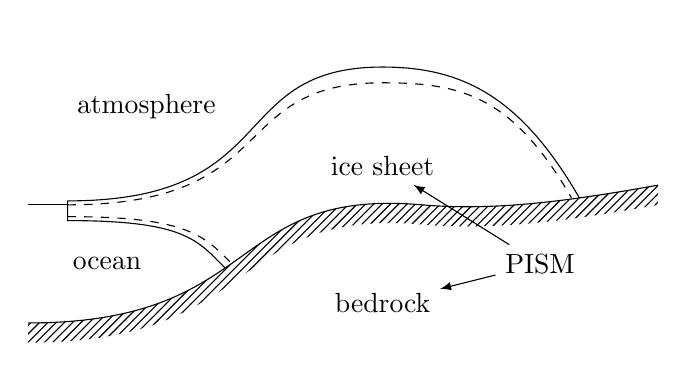
\begin{tikzpicture}[>=latex]

% white background
\fill[white] (0,0) rectangle +(8,4);
%\draw [help lines, lightgray] (0,0) grid (8.0,4.0);

% grounding line and inland margin coordinates
\coordinate (cf) at (0.5, 1.75) ;
\path[name path=xgl] (2.5,0) -- +(0,4) ;
\path[name path=xim] (7,0) -- +(0,4) ;

% bedrock topography
\draw [name path=bed]
    (0,0.25) .. controls +(0:3) and +(-5:-2.5) ..  (5,1.75)
	  .. controls +(-5:1) and +(10:-1) .. (8,2);
\fill [pattern=north east lines]
    (0,0.25) .. controls +(0:3) and +(-5:-2.5) ..  (5,1.75)
	  .. controls +(-5:1) and +(10:-1) .. (8,2)
	  -- +(0,-0.25)
          .. controls +(10:-1) and +(-5:1) .. (5,1.5)
          .. controls +(-5:-2.5) and +(0:3) .. (0,0);

% locate the grounding line
\path [name intersections={of=bed and xgl, by=gl}] ;
\path [name intersections={of=bed and xim, by=im}] ;

% surface topograpy
\draw [name path=surf]
    (cf) -- +(0,0.05)
         .. controls +(0:2.75) and +(0:-2) .. (4.5, 3.5)
         .. controls +(0:1) and +(-60:-1.5) .. (im);
\draw [dashed]
    (cf) .. controls +(0:2.75) and +(0:-2) .. (4.5, 3.3)
         .. controls +(0:1) and +(-60:-1.5) .. ($(im)-(0:0.1)$);

% ice shelf base
\draw [name path=base]
    (cf) -- +(0,-0.2)
         .. controls +(0:1.5) and +(135:0.5) .. (gl) ;
\draw [dashed]
    ($(cf)+(0,-0.15)$)
         .. controls +(0:1.5) and +(135:0.5) .. ($(gl)+(45:0.1)$) ;

% sea level
\draw [name path=sl] (cf -| 0,0) -- (cf) ;


\node (atm) at (1.5, 3) {atmosphere};
\node (ice) at (4.5, 2.25) {ice sheet};
\node (ocn) at (1, 1) {ocean};
\node (bed) at (4.5, 0.5) {bedrock};

\node (pism) at (6.5, 1) {PISM};
\draw[->] (pism) -- (ice);
\draw[->] (pism) -- (bed);

\end{tikzpicture}
\end{document}
